\subsection{Esquemas de navegabilidad del sistema de inclusión}
\begin{itemize}
  \item \textbf{Inclusion de partidas}
  \begin{figure}[H]
    \centering
    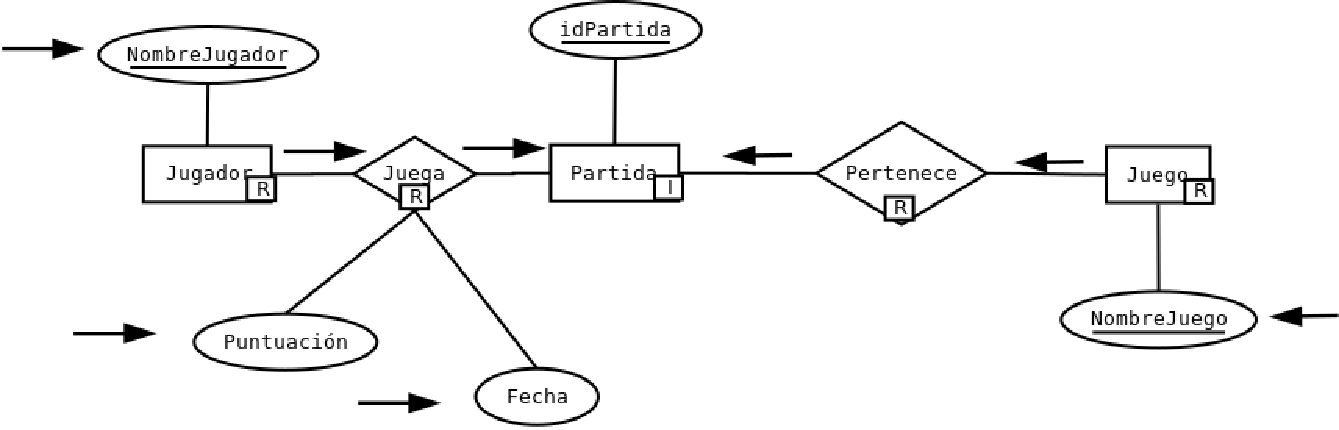
\includegraphics[width=0.5\linewidth]{../Diagramas/pdf/IncluirPartida.pdf}
    \caption{Esquema de navegabilidad de del proceso 1}
  \end{figure}

  \item \textbf{Modificación de partidas}
  \begin{figure}[H]
    \centering
    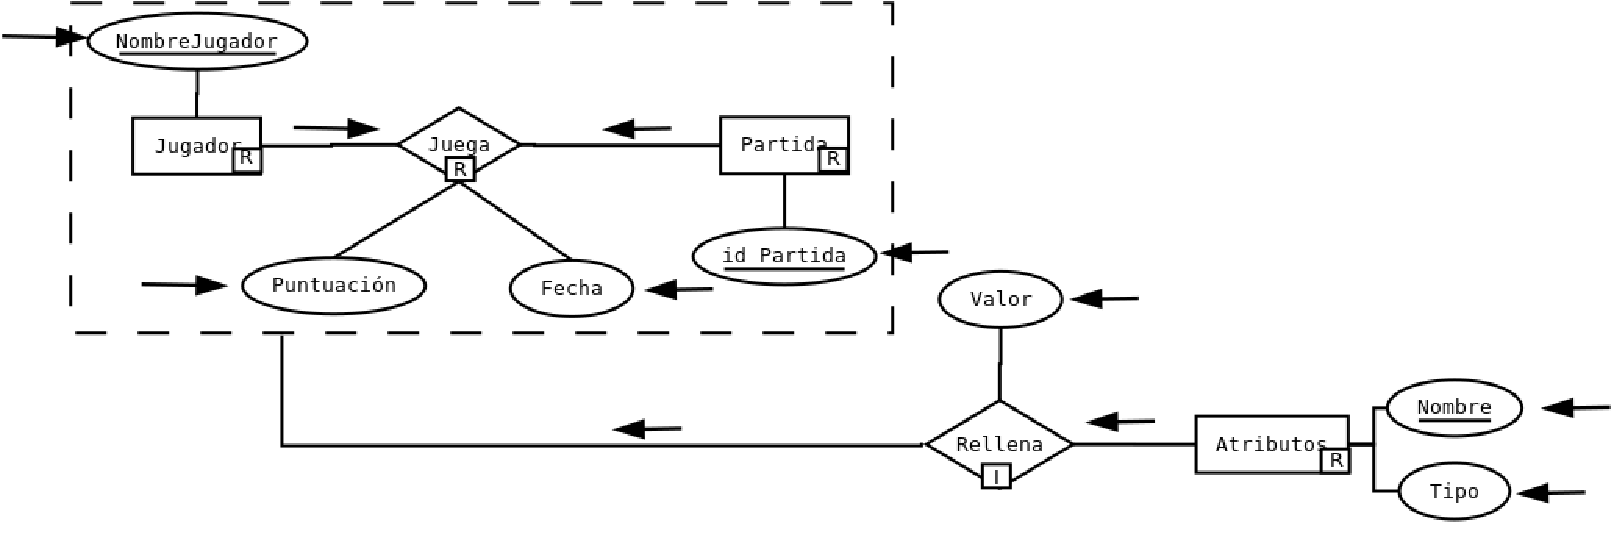
\includegraphics[width=0.5\linewidth]{../Diagramas/pdf/ModificarPartida.pdf}
    \caption{Esquema de navegabilidad del proceso 2}
  \end{figure}

  \item \textbf{Eliminación de partidas}
  \begin{figure}[H]
    \centering
    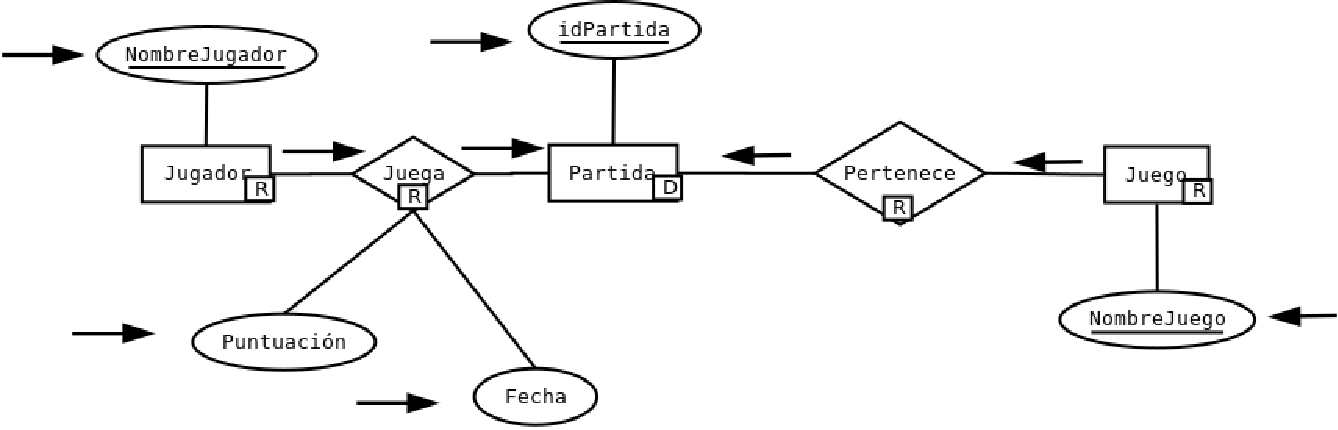
\includegraphics[width=0.5\linewidth]{../Diagramas/pdf/EliminarRegistro.pdf}
    \caption{Esquema de navegabilidad del proceso 3}
  \end{figure}

  \item \textbf{Comentar la partida de otro jugador}
  \begin{figure}[H]
    \centering
    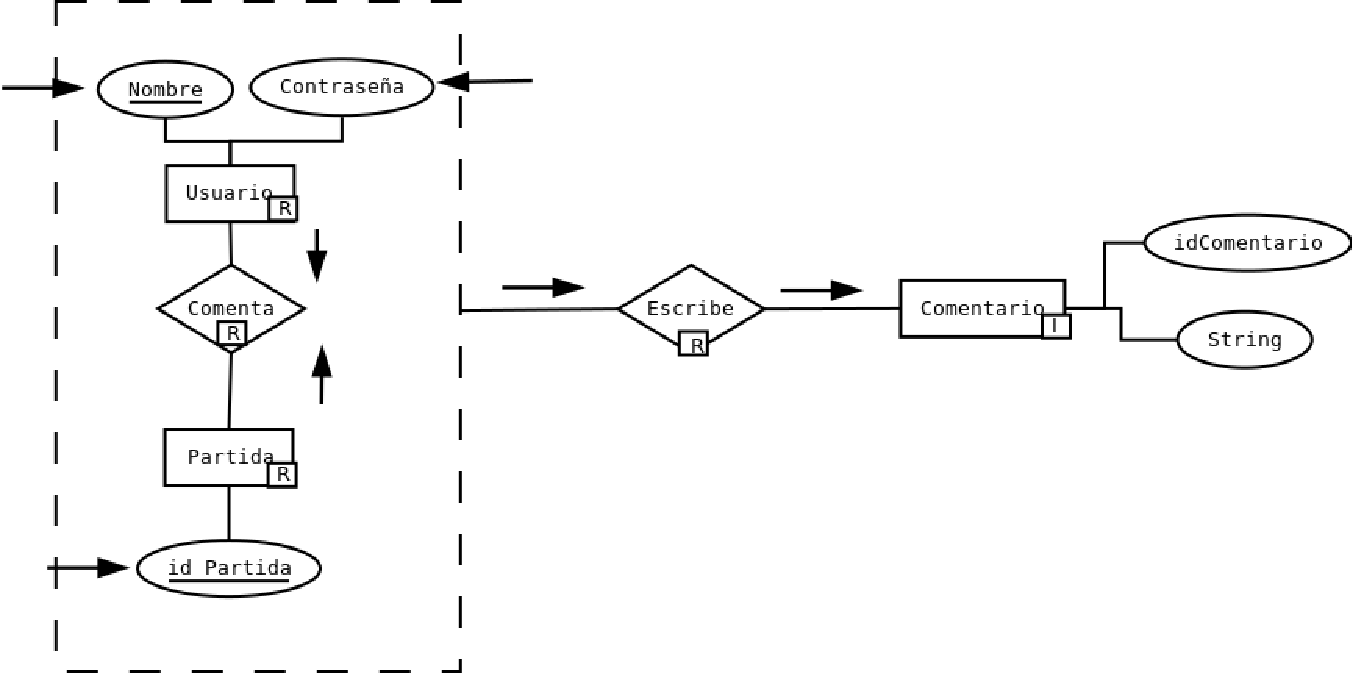
\includegraphics[width=0.5\linewidth]{../Diagramas/pdf/ComentarPartida.pdf}
    \caption{Esquema de navegabilidad del proceso 4}
  \end{figure}


\end{itemize}
